\documentclass{report}
\usepackage[utf8]{inputenc}
\usepackage{natbib}
\usepackage{graphicx}
\usepackage[pagestyles]{titlesec}
\usepackage{pdfpages}

\title{Design Document}
\author{AmorosiniCasaliFioravanti}
\date{December 2019}

\titleformat{\chapter}[display]{\normalfont\bfseries}{}{0pt}{\Huge}
\newpagestyle{mystyle}
{\sethead[\thepage][][\chaptertitle]{}{}{\thepage}}
\pagestyle{mystyle}

\begin{document}


\includepdf[pages={1}]{./img/FrontPage}

\chapter{Introduction}
\section{Purpose}
While the RASD presented a general view of the SafeStreets appliction and its features, this document aims to further analyze the system's design and architecture, as well as describing for each of its components their runtime behaviour, integration, interfaces, implementation and testing plans.
This document is mainly intended to be used by the test and development teams as a guidance in the development process, but also to prevent structural degradation during maintainance and extension phases. Nonetheless, the document is also addressed to all the stakeholders who are interested in supervising the development process.

\section{Scope}
SafeStreets: an application that aims to improve the safety of urban areas by giving its users the possibility to report traffic violations to authorities. Users are logged in either as citizen, those who report the violations, and authorities, those who are notified about newly reported violations and are supposed to take action on them.\\
The system is in charge of collecting all the reports, storing them, and notifying the authorities about them. The stored reports are then used to build statistics, find unsafe areas, and compute suggestions on how to improve the safety of such areas. The system may also communicate with local Municipalities' Systems in order to retrieve information about accidents and iussued traffic ticket: in this case some of the above functions are enhanced, and some new functions are enabled (g.e computing statistics on traffic ticked).\\
\newline
Further information about the scope of the application can be found in the Chapter 1 of the RASD.

\section{Definitions, Acronyms and Abbreviations}
\subsection{Definitions}
\begin{itemize}
    \item \textit{Client}: a piece of computer hardware or software that accesses a resource or a service made available by a Server.
    \item \textit{Server}: a device or a computer program that provides resources or functionalities to other programs or devices.
    \item \item \textit{Safety Suggestion}: recommendation to improve the safety of urban areas. It is computed by analyzing the statistics built by the system.
    \item \textit{Firewall}: a network security systems that monitors incoming and outcoming network traffic, applying predefined predefined security rules.
\end{itemize}
\subsection{Acronyms}
\begin{itemize}
    \item \textbf{RASD}: \textit{Requirement Analysis and Specification Document}, the document in which all the requirements and goals of the application are throughly described.
    \item \textbf{API}: \textit{Application Programming Interface}, interface, or communication protocol between Client and Server intendend to simplify the building of the Client-side software.
    \item \textbf{GPS}: \textit{Global Positioning system}, technology widely used to get the user's position.
    \item \textbf{DBMS}: \textit{Data Base Management system}, software that provides organized space memory to store information.
    \item \textbf{OCR}: \textit{Optical Character Recognition}, software dedicated to the detection of characters contained in a document and to their transfer to digital text that can be read by a machine. In this context, OCR will be used to read license plates.
    \item \textbf{UML}: \textit{Unified Modeling Language}, a standard visual modeling language intended to be used for analysis, design, and implementation of software-based systems.
    \item \textbf{MVC}: \textit{Model View Controlles}, a software design pattern commonly used to provide user interfaces.
    \end{itemize}
\subsection{Abbreviations}
\begin{itemize}
    \item {[R$_{i}$]}: i-th requirement.
    \end{itemize}
\section{Reference Documents}
\begin{itemize}
    \item Specification document: \textit{SafeStreets Mandatory Project Assignment.pdf}.
    \item Requirement Analysis and Specification Document: \textit{RASD.pdf}.
\end{itemize}
\section{Document Structure}
This document is presented as it follows:
\begin{enumerate}
    \item \textbf{Introduction} presents a general overview, the scope and the purpose of the document.
    \item \textbf{Architectural Design} shows the main components of the system and their relationships. This section will also discuss the architectural choices of the design process.
    \item \textbf{Algorithm Design} presents and discusses the algorithms that will enable the system's functionalities.
    \item \textbf{user Interface Design} provides some further details on the user interface defined in the RASD.
    \item \textbf{Requirement Traceability} maps all the functional requirements defined in the RASD over the components that will accomplish them.
    \item \textbf{Implementation, Integration and Testing Plans} shows the order in which the implementation and the integration of the components will occur, and how the testing phase will be carryed out.
    \item {\textbf{Effort spent}} displays the time spent writing this document by each member of the team.
\end{enumerate}
\chapter{Architectural Design}
\section{Overview}
In this chapter the architectural structure of the system will be discussed at multiple levels of abstraction. A high-level view of the components and their interactions is represented in Figure \ref{fig:overview}. The details will be explained in the next sections.
\begin{figure}[!ht]
	\begin{center}
	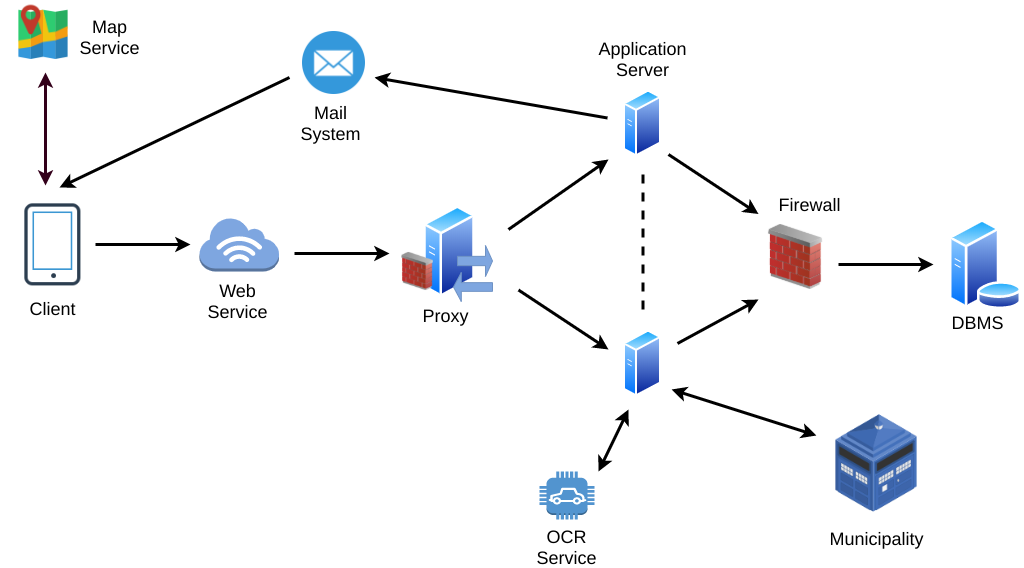
\includegraphics[width=\textwidth]{img/HighLevelOverview.png}
    \end{center}
    \label{fig:overview}
	\caption{High-level overview of the system.}
\end{figure}
\newpage
\section{Component view}
The UML component diagram aims at capturing the internal modular structure of the components, showing how they are connected together in order to form larger components. Components are wired together by using an assembly connector to connect the required interface of one component with the provided interface of another component.
\begin{figure}[!ht]
	\begin{center}
	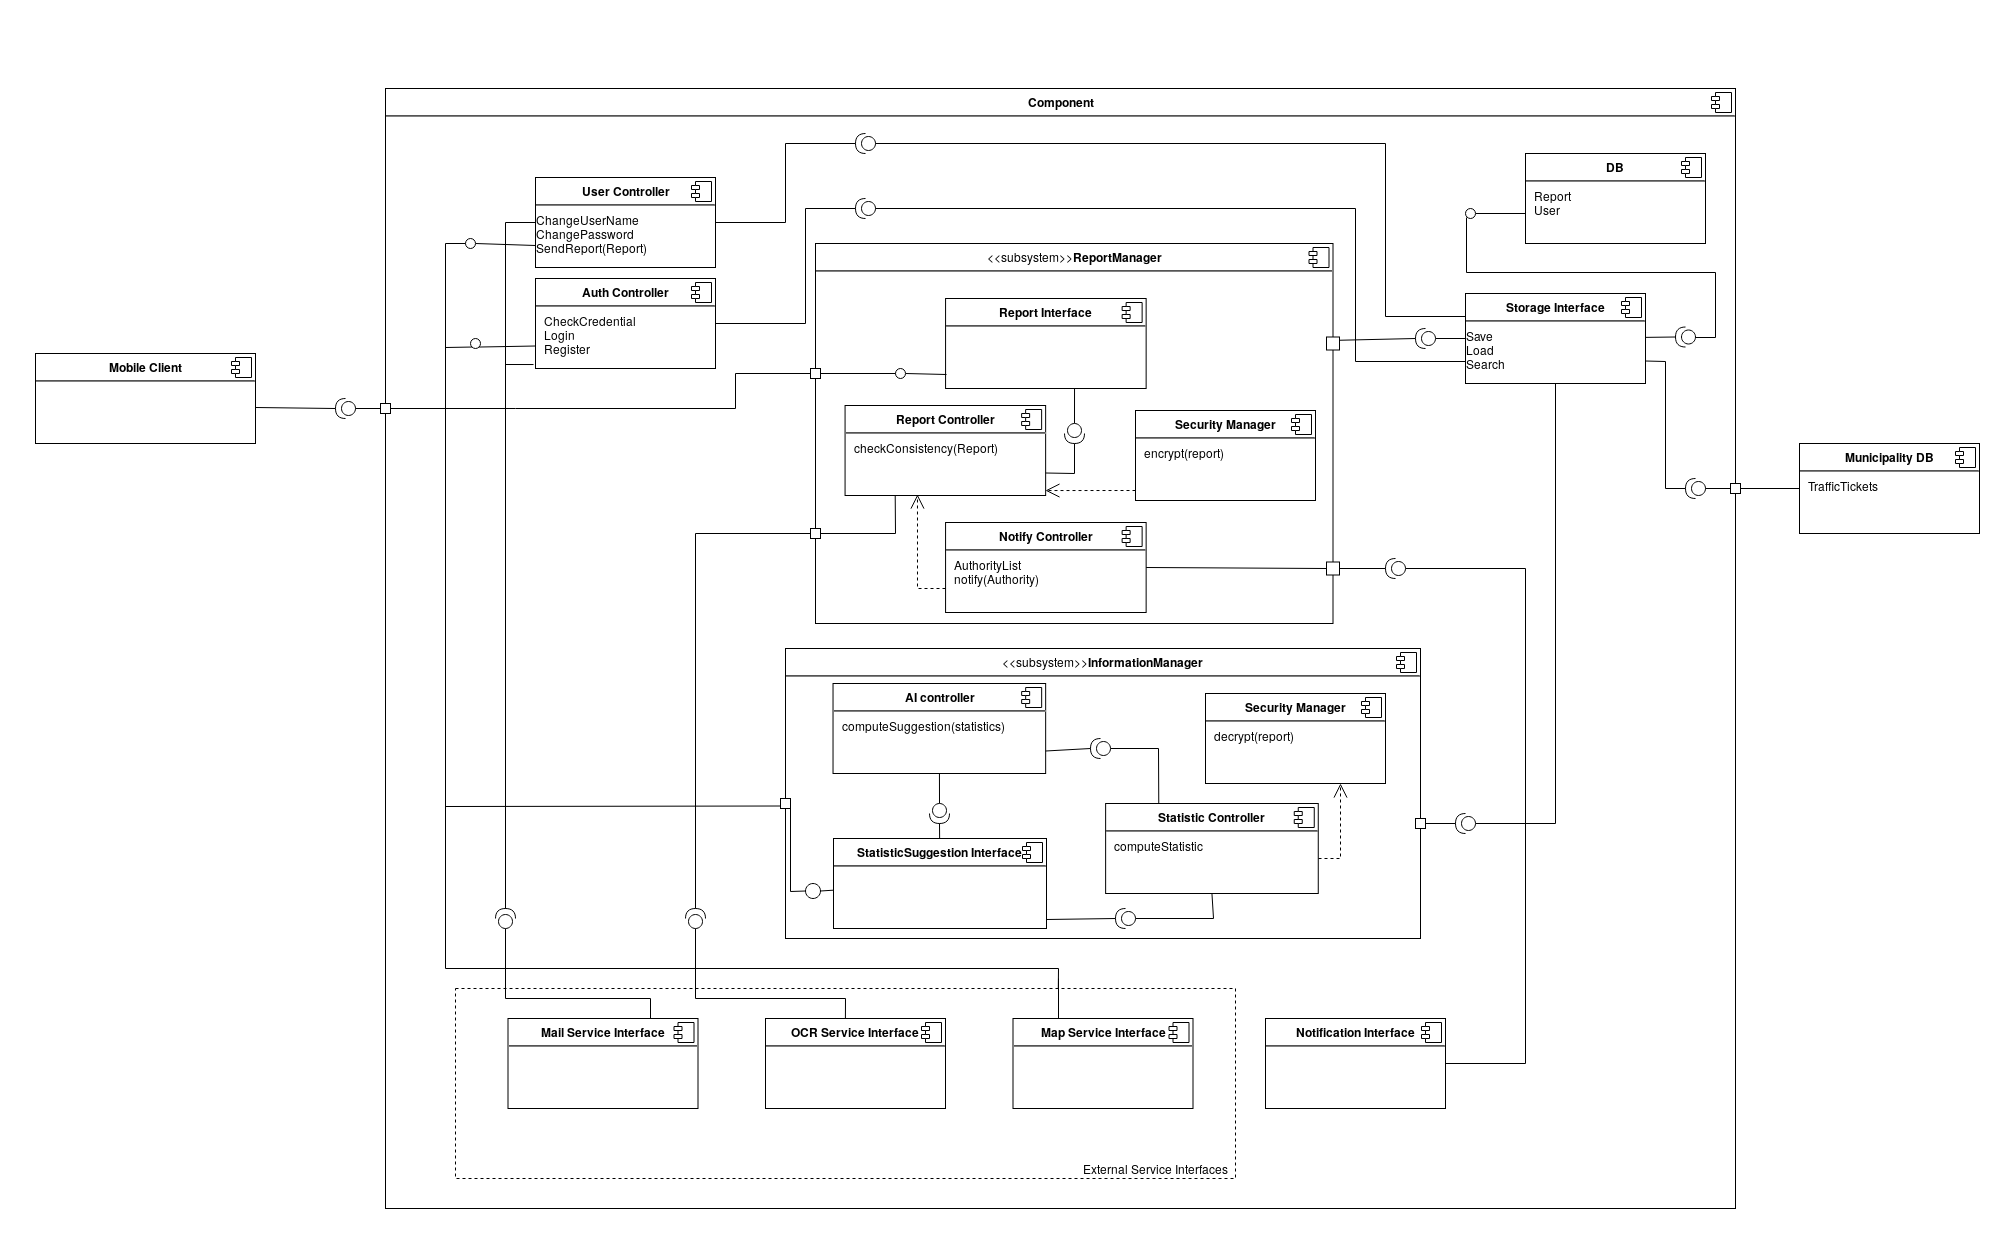
\includegraphics[width=\textwidth]{img/ComponentDiagram1.png}
    \end{center}
    \label{fig:componentdiagram}
	\caption{Component diagram of the system.}
\end{figure}
Below is a description of each component:
\begin{itemize}
\item \textbf{Mobile Client}: the client device that accesses to the functionalities of the entire system. It is implemented as thin client as explained below.
\item \textbf{User Controller}: it takes care of all the operation related to the user's data. It exposes methods to change account credentials and it stores the user's data in the database using the Storage Interface.
\item \textbf{Auth Controller}: it takes care of all the authentication-related operations: it is responsible both for the log in and the registration process, and it also uses the \textit{Storage Interface} to retrieve and store new users' credentials in the databse. During the registration process, the Auth Controller uses the \textit{Mail Service Interface} to communicate with the Mailing Service in order to send registration emails.   
\item \textbf{Report Manager}: it's a \textit{subsystem} component in charge of all the processing functions on the newly recieved reports:
\begin{itemize}
    \item \textbf{Report Interface}: it exposes to the User an interface in the form of a blank report to be compiled.
    \item \textbf{Report Controller}: it aims to check the consistency of the report sent. To do this it uses the Report Interface to know how the report form is and how the report sent has been compiled.
    \item \textbf{Notify Controller}: the role of this component is to notify the correct authorities based on their municipality, using his \textit{AuthorityList}. It depends on the Report Controller, in the sense that it will notify the authorities only if the check of the report is successful and the type of the report is \textit{Traffic Violation}.
    \item \textbf{Security Manager}: it takes care of the security side: as specified in the Security section of the RASD, before being stored, the report is encrypted and then stored in the database. This task is accomplished by this specific component, that also depends on the Report Controller due to the fact that if the report doesn't pass the check verification, it will be discarded and therefore never encrypted.
\end{itemize}
\item \textbf{Information Manager}: a \textit{subsystem} in charge of building statistics, compute safety suggestions and deploy them to the users who requested them.
    \begin{itemize}
        \item \textbf{StatisticsSuggestions Interface}: it exposes to the users the latest statistics and safety suggestions. As aready mentioned in the RASD, the exposed data may be different according to the level of visibility granted to different users.
        \item \textbf{Statistics Controller}: it analyzes the stored reports to build statistics and find unsafe urban areas. Depending on the agreements with local municipalities, this component can also compute statistics on iussued traffic tickets or refine its statistics about accidents.
        \item \textbf{AI Controller}: its role is to analye previously built statistics and compute safety suggestions. These suggestions are addressed to the authorities who use SafeStreets application.
        \item \textbf{Security Manager}: similarly to the one described in the Report Manager subsystem, this component is in charge of decrypting stored reports so that they can be analyzed. To ensure that no report is ever altered, this component can perform read-only operations, whereas the one in the Report Manager is the ony one which disposes of write permissions.
    \end{itemize}
\item \textbf{Storage Interface}: its main purpose is to retrive the reports from the database, decopuling the other components of the system from the particular data sources. This component is also in charge of authenticating the system with local municipalities' systems, and eventually crossing their data with SafeStreets' own information.
\item \textbf{DB}: this component represent the DBMS, which provides an interface to read and store data. In the database both user credentials and submitted reports are stored.
\item \textbf{External Services Interfaces}: it's a set of components whose main task is to make an API call to the corresponding third party service.
    \begin{itemize}
        \item \textbf{Mail service Interface}: 
        \item \textbf{OCR service Interface}: it calls a service used by the Report Manager to read license plates from pictures submitted in the reports by users.
        \item \textbf{Map service Interface}: it provides the users with the functionality of visualizing the statistics (and their own position) on a geographic area using an interactive map.
\end{itemize} 
\end{itemize}
\section{Deployment view}
In this section it is described the deployment view of the components inside the system.
The deployment diagram describes the distribution of components of the hardware.
\begin{figure}[!ht]
	\begin{center}
	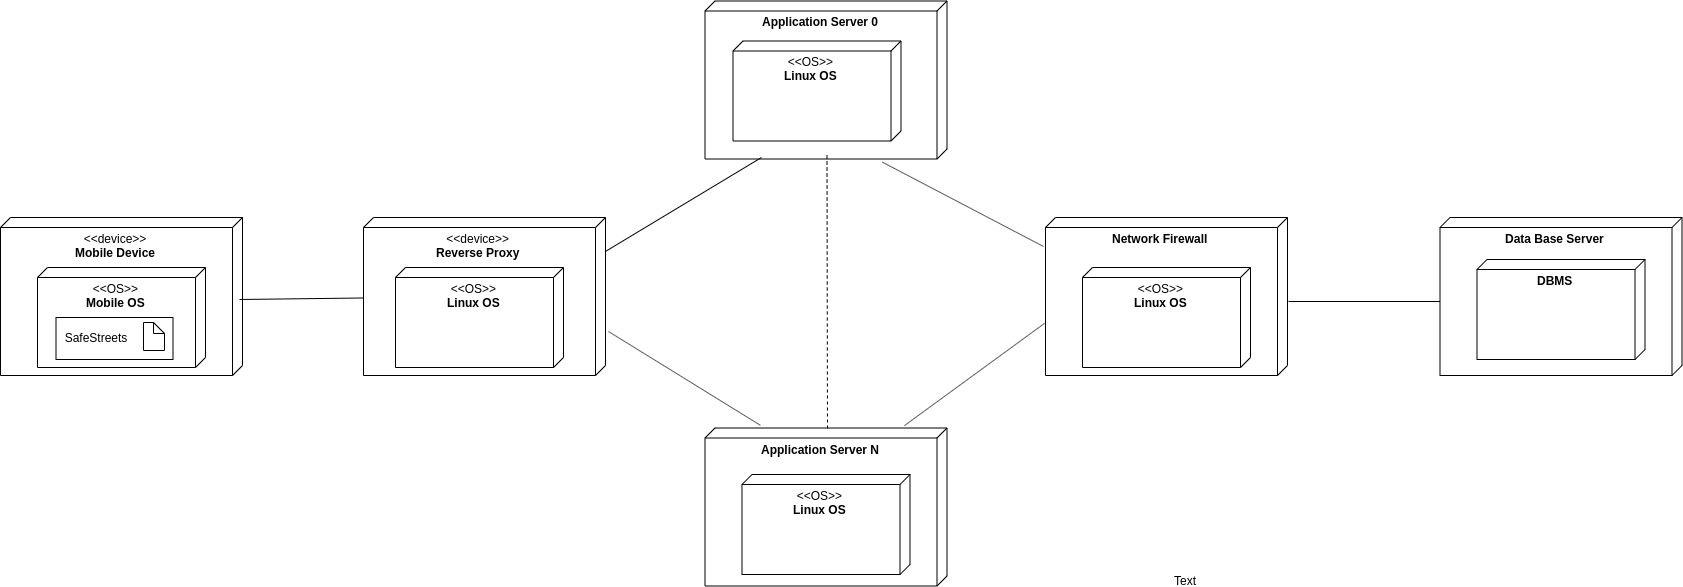
\includegraphics[width=\textwidth]{img/DeploymentView.png}
    \end{center}
    \label{fig:deploymentview}
	\caption{Deployment diagram of the system.}
\end{figure}\\
The system is composed of a multitier architecture, each specific role is clarified below.\\
\begin{itemize}
    \item \textbf{Client}\\
    The first tier contains the client mobile machines which have installed SafeStreets application
    to access all its functionalities.\\
    \item \textbf{Reverse Proxy}\\
    The second tier contains a reverse proxy to implement load balancing on the several requests to access the application servers.
    Furthermore, it is a cacheble component who can speed-up the most frequent requests.
    Linux machine have been chosen for safety and simplicity. \\
    \item \textbf{Application servers}\\
    This is the middleware level of the application where all the computations happen. The servers
    are distributed to increase the scalability of the network, they are also part of the second tier.\\
    \item \textbf{Firewall}\\
    The access to the Database is protected from a firewall to avoid unauthorized accesses to sensible data.\\
    \item \textbf{Database Server}\\
    This is the last layer of the architecture. All the data are stored here structured in a relational DBMS.
\end{itemize}

\section{Runtime view}

\section{Component interfaces}

\section{Selected architectural	styles and patterns}
The following architectural patterns are used to build the structure of the system in order to provide all the services of SafeStreets application.\\

\begin{center}\large{\textbf{Client-Server Architecture}}\end{center}
Client-Server architecture is a computing model that features two roles: a Server that hosts, delivers and manages most of the resources and services, and a Client which exploits them.
\begin{center}\large{\textit{Motivations}}\end{center}
\noindent This structure provides several advantages:
\begin{itemize}
    \item Scalability and Mantainability: it is possible to repair or add more resources to the architecture without significative service interruptions.
    \item Security: the server is able to manage what levels of access each user can have with respect to specific resources.
\end{itemize}\vspace{2mm}

\begin{center}\large{\textbf{Three-tiered Architecture}}\end{center}
This type of architecture is a kind of Client-Server paradigm where three tiers are phisically separated:
\begin{itemize}
	\item The \textit{presentation tier} is the top-most level of the architecture, which provides an interface that users can use to directly access the application. 
	It is the top-most tier and the only one accessible from the Client.
	\item The \textit{application tier} runs the business logic of the application and executes functions that elaborate data. 
	A Reverse Proxy is needed to handle the Client requests and to balance the workload, the requests are forwarded to 
	the application serves in order to provide the right data.
	\item The \textit{database tier} includes the data persistence mechanisms and the data access layer that encapsulates 
	the persistence mechanisms and exposes the data.
\end{itemize}
\begin{center}\large{\textit{Motivations}}\end{center}
A multi-tier application architecture provides a model with several advantages: in this way developers can create flexible and reusable 
applications that can be modified, enhanced or maintained just by operating on a specific layer, instead of reworking the entire application. Furthermore, a general multitier architecture can also help improve the development efficiency by allowing teams to focus on their core competencies.

\begin{figure}[!ht]
	\begin{center}
	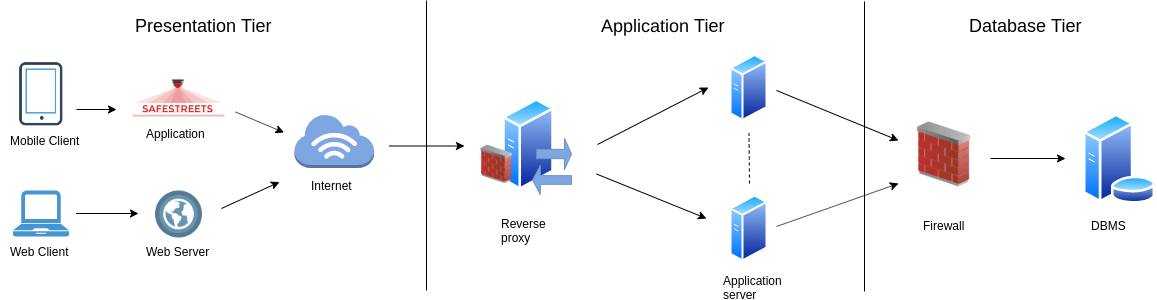
\includegraphics[width=\textwidth]{img/TiersArchitecture.png}
	\end{center}
	\caption{Three-tier architecture schema.}
\end{figure}

\begin{center}\large{\textbf{Thin Client}}\end{center}
A thin Client is a lightweight computer which does most of the computation in a remote Server. In this paradigm in fact, since the Servers take care of several duties such as storage 
of data and performing calculations, the Client does not need to have a large memory or powerful computing capabilities to run the application.
\begin{center}\large{\textit{Motivations}}\end{center} 
The application is thought for mobile phones which do not have great computing power or very large memories. Thanks to a thin client a internet connection is virtually the only requirements to use the application. Furthermore, this architecture simplify the front-end implementation by shifting most of the execution to the servers.

\begin{center}\large{\textbf{MVC Design Pattern}}\end{center}
Model-View-Controller is a software design pattern commonly used to develop user interfaces. Indeed, this pattern is used for the front-end implementation of the application. It divides the program logic in three interconnected elements: \textit{model} that directly manages data and rules of the application, \textit{view} which handles any representation of data, \textit{controller} that 
accepts input and converts it to commands for the model or view. This mechanism is used to separate internal representation of information from the ways information is presented to and accepted from the user. \\
\begin{center}\large{\textit{Motivations}}\end{center} 
MVC allows full encapsulation of objects. This means that each component can be changed without creating issues to other components.
Furthermore, MVC provides decopuling of its components, which means that developers are able to work in parallel on different components of the pattern without interfering with each other.

\begin{center}\large{\textbf{Reverse Proxy Design Pattern}}\end{center}
A simple proxy acts as an interface to refer an object in another machine. The reverse proxy offers a single point of access (with HTTP) to multiple Clients who want to access to several application servers. In practice, it is a wrapper for an object behind the scenes. 
Proxies also provides extra functionalities such as data caching (g.e. store the newest statistics available) and security (g.e. client-side firewall).\\
\begin{center}\large{\textit{Motivations}}\end{center} 
It is useful to organize the requests of multiple clients and to save frequent requested informations. It also protects the application servers from external attack and slightly improve the overall performances.

\end{document}